\subsubsection{分析与准备：为何保留界面反射场}

本节先处理一个边界问题：问题一究竟应当把哪些返回光写进模型。条纹峰距只反映传播相位的变化，若折射率随波数变化而又没有标定，直接把峰距换成几何厚度就会把材料光学性质误当成厚度；因此主路线需要同时保留入射角、色散和偏振，而不是先填入一个固定折射率。

实测输入沿用第\ref{sec:common-coordinates}节的共同坐标，光学缺项见第\ref{sec:optical-inputs}节。两种角度改变了光线在外延层中的传播方向，却没有改变同片几何厚度；这使双角可以共同约束一条厚度参数，同时保留各自的界面振幅。直接采用全谱同型峰距并配固定折射率的尝试，正是因为这些输入缺失而被改为使用“波数乘纵向传播因子”的色散坐标。
% src:求解/问题1/结果/实测输入核验.json:共同原始波数点数;波数范围_每厘米
% src:交接/实验记录.json:26.现象;26.决定

两束边界由题面限定为表面直接反射和首个返回，后续往返不在本问提前叠加。图\ref{fig:once-return}把空气、外延层与衬底、外部入射角、层内传播方向和厚度路径放在同一几何关系中；所谓“双束界面场反演”，就是由这两束光的复场叠加计算反射率，再寻找使计算值与观测值接近的厚度。这样既保留了$10^\circ$与$15^\circ$的角度差异，也为问题三比较高阶返回留下清晰的基准。

\begin{figure}[H]
  \centering
  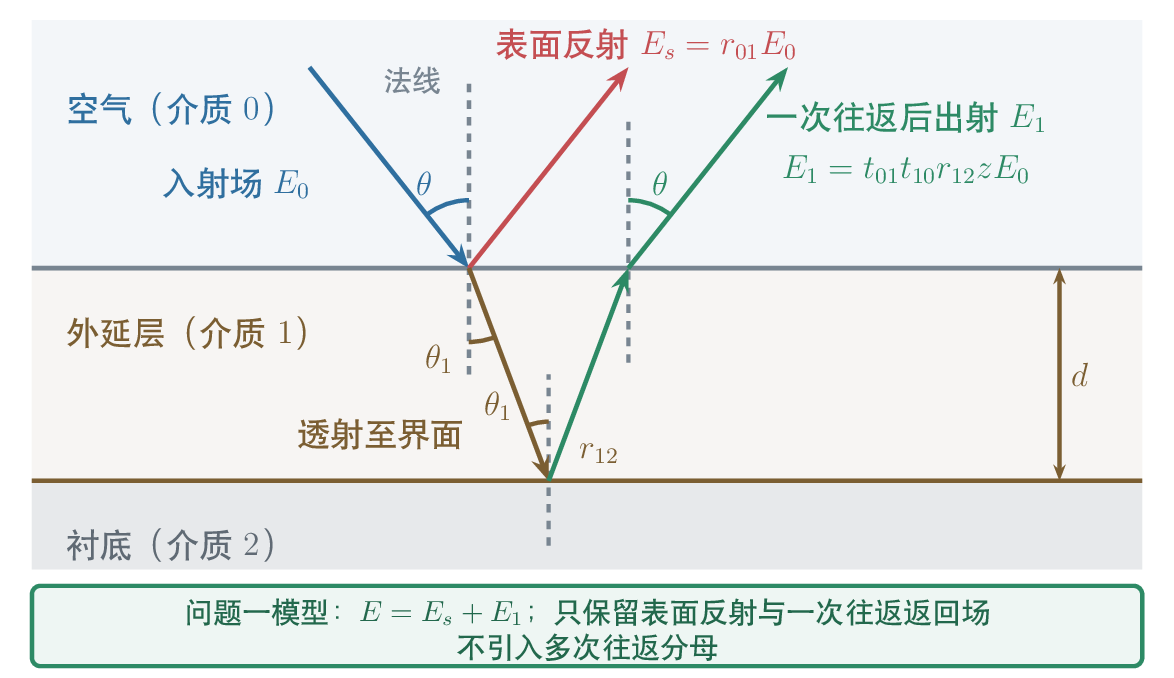
\includegraphics[width=0.8\textwidth]{../求解/问题1/图片/一次往返保留两束反射场.png}
  \caption{一次往返的两束反射场路径}
  \label{fig:once-return}
\end{figure}

路线选择也由同口径对照决定。已知光学参数的24组原型双角合成案例中，双束界面场反演的平均相对误差为$0.0010\%$，低于色散峰序反演的$0.0201\%$和连续相位拟厚的$0.0041\%$；逐观测输入一致的结论限定于这三个已核验原型，故没有把不同路线的结果平均，而是将后两者保留为级次与相位的独立核对。色散峰序反演按折射率变化修正峰谷位置，再按条纹级次求厚度；连续相位拟厚则沿波数展开条纹相位，由相位变化反推厚度。误差以合成光谱的已知厚度为参照，比较各路线在匹配生成机制下的回收表现。
% src:求解/问题1/原型结果/路线2.json:主指标值;已完成例数
% src:求解/问题1/原型结果/路线1.json:主指标值
% src:求解/问题1/原型结果/路线3.json:主指标值
% src:交接/锦标赛核验_问题1.json:共同输入核对
% src:交接/实验记录.json:66.现象;66.决定

正式复算另用一组生成观测，主方法平均误差为$0.0008\%$，与它使用相同输入的峰距基线为$2.59\%$；原型与正式组的含噪观测不同，二者不能拼成一组路线排名。
% src:求解/问题1/结果/合成验证.json:主指标.数值;常折射率峰距基线.平均绝对相对误差_百分比

强度形状进一步排除了“全谱恒幅条纹”的简化：附件1在$500$--$1000\ \mathrm{cm}^{-1}$和$3000$--$3500\ \mathrm{cm}^{-1}$两个诊断波段的反射率标准差分别为$28.9$和$0.189$个百分点，散布尺度相差悬殊。故主求解直接拟合两束截断场展开后的强度，局部极值和峰距承担相位解释与级次核对；下一节将从两束截断场推导偏振强度、色散相位及条纹间距。
% 依据:交接/建模笔记_问题1.md:4.强度展开、色散和峰谷系数
% src:交接/实验记录.json:27.现象;27.决定
